%% Beispiel-Präsentation mit LaTeX Beamer im KIT-Design
%% entsprechend den Gestaltungsrichtlinien vom 1. August 2020
%%
%% Siehe https://sdqweb.ipd.kit.edu/wiki/Dokumentvorlagen

%% Beispiel-Präsentation
\documentclass[en]{sdqbeamer} 
 
%% Titelbild
\titleimage{banner_2020_kit}

%% Gruppenlogo
\grouplogo{} 

%% Gruppenname und Breite (Standard: 50 mm)
\groupname{Institute for Automation and Applied Informatics (IAI)}
%\groupnamewidth{50mm}

% Beginn der Präsentation

\title[ABAC for Substations]{Attribute-Based Access Control for Substations (ABAC-SS)}
\subtitle{Master's Thesis Proposal} 
\author[Moritz Gstuer]{Moritz Gstuer}

\date[06.\,06.\,2024]{06. June 2024}

% Literatur 
 
\usepackage[citestyle=authoryear,bibstyle=numeric,hyperref,backend=biber]{biblatex}
\addbibresource{../bibliography/masterthesis.bib}
\bibhang1em

\begin{document}
 
%Titelseite
\KITtitleframe

%Inhaltsverzeichnis
\begin{frame}{Agenda}
\tableofcontents
\end{frame}

\section{Motivation}
\begin{frame}{Motivation}
    Motivation Figure
\end{frame}

\section{System Model}
\begin{frame}{Substation Automation System (SAS)}
    \centering
	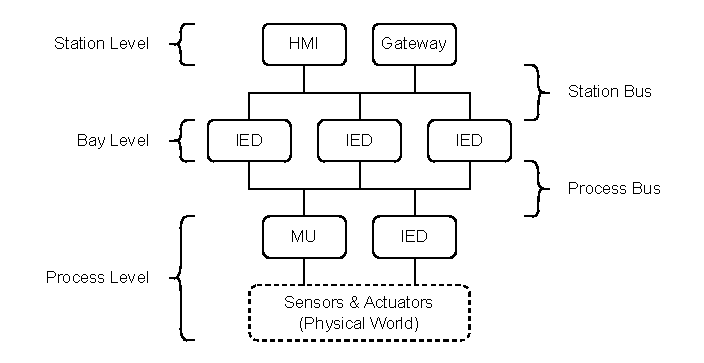
\includegraphics[width=0.8\textwidth]{./figures/substation_architecture.drawio.pdf}
\end{frame}

\begin{frame}{SAS Communication}
    \begin{blueblock}{Station Bus}
        Transport-Layer-based Session-oriented Communication (e.g. MMS Protocol)
        \\$\rightarrow$ Client-Server (Unicast)
    \end{blueblock}
    \begin{blueblock}{Process Bus}
        Data-Link-Layer-based Message-oriented Communication (e.g. GOOSE \& SV Protocol)
        \\$\rightarrow$ Publisher-Subscriber (Broadcast/Multicast)
    \end{blueblock}
    \begin{grayblock}{IEC 61850 Message Types \& Performance Classes}
        Requirements for messages in substations
        \\Examples: GOOSE (Type 1A, 3ms), SV (Type 4, 3ms), MMS (Type 2/3/5, 100-10000ms)
    \end{grayblock}
    TODO Cite IEC 61850-5 and -8
\end{frame}

\begin{frame}[allowframebreaks]{Requirements \& Constraints}
    \begin{columns}
        \column{.5\textwidth}
        \begin{blueblock}{Security}
            \begin{itemize}
                \item Confidentiality
                \item Integrity
                \item Authenticity
                \item Non-Repudiation
                \item Least Privilege Principle (PoLP)
                \item Separation of Duties (SoD)
                \item Privacy-Preservation
            \end{itemize}
            $\rightarrow$ Encryption, Authentication, \& Authorization
        \end{blueblock}
        \column{.5\textwidth}
        \begin{blueblock}{Performance}
            \begin{itemize}
                \item Soft \& Firm Real-Time
                \item CPU \& Memory
                \item Energy \& Power
            \end{itemize}
            $\rightarrow$ Separation of Concerns \& Modularity
        \end{blueblock}
        \begin{blueblock}{Interoperability}
             Existing Inter-/Intra-SAS Protocols \& SCADA Systems
             \\$\rightarrow$ Compatibility \& Interchangeability
        \end{blueblock}
    \end{columns}
    \framebreak
    \begin{redblock}{Overarching Requirements for Operational Technology (OT)}
        \begin{itemize}
            \item Availability
            \item Safety
        \end{itemize}
        Under any Circumstances: Continuing \& Safe Operation
        \\$\rightarrow$ Fail-Operational before Fail-Safe
    \end{redblock}
\end{frame}

\section{Related Work}
\begin{frame}{Related Work}
    Message Authentication, Asym. Performance Evaluation, BitW- \& HW-Solutions, Access Control
\end{frame}

\begin{frame}{Research Questions}
    Research Questions
\end{frame}

\section{Proposed Approach: SAZE}
\begin{frame}{SAZE ("Sassy") Approach}
    \begin{greenblock}{\textbf{S}erver-aided \textbf{A}BAC with \textbf{Z}ero-RTT \textbf{E}ncryption (SAZE)}
        \begin{itemize}
            \item Mandatory Access Control \& Encryption for SAS Communication
            \item Transparent Security for IEC 61850 Devices (e.g. IED \& MU)
        \end{itemize}
    \end{greenblock}
    %Overview: Describe parts Server-Aided Attribute-Based Access Control (Including Authentication and Authorization Delegation) with Zero-RTT Encryption (Asym./Sym.)
\end{frame}

\begin{frame}{SAZE Components}
    \centering
	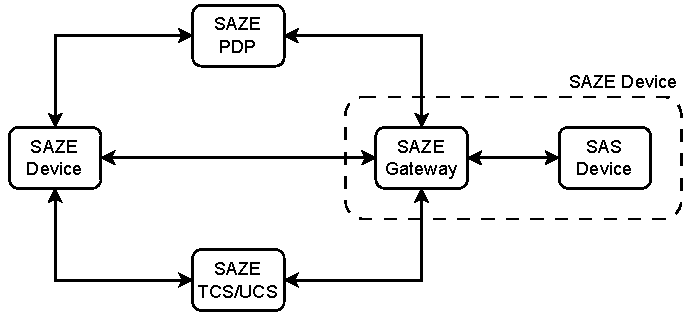
\includegraphics[width=0.8\textwidth]{./figures/saze_components.drawio.pdf}
\end{frame}

\begin{frame}{SAZE SAS Architecture}
    \centering
    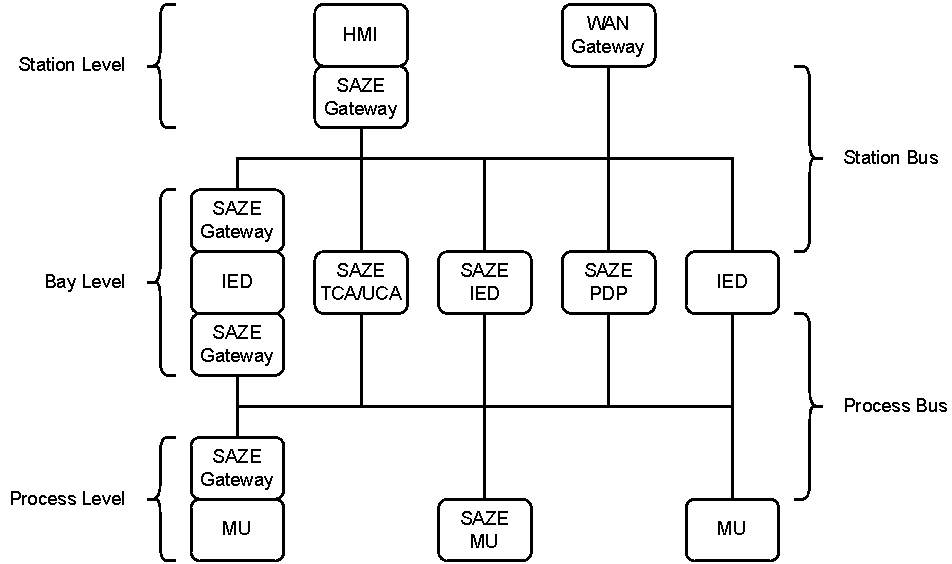
\includegraphics[height=0.75\textheight]{./figures/saze_architecture.drawio.pdf}
\end{frame}

\subsection{Server-Aided ABAC}
\begin{frame}{Attribute-Based Access Control (ABAC)}
    ABAC Definition
    ABAC Benefit vs. traditional IBAC/RBAC solutions including RT-Attribute like network congestion
    ABAC Requirements -> Authentication \& Authorization
\end{frame}

\begin{frame}{Authorization, Authentication, \& Access Control}
    \centering
	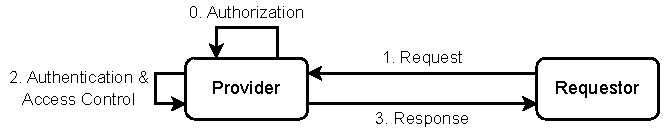
\includegraphics[width=0.9\textwidth]{./figures/access_control_request_traditional.drawio.pdf}
    \begin{redblock}{Problem}
        TODO
        Device responsible for policy management, policy enforcement, access control decisions, authentication of requestor\dots
    \end{redblock}
\end{frame}

\begin{frame}{Server-Aided ABAC}
    ABAC Problem -> Performance/Computational Effort/Certificates for Attributes\dots
    Idea -> Authentication and Authorization Delegation to Server => "Server-Aided ABAC"
\end{frame}

\begin{frame}{Server-Aided ABAC}
    Figure with authentication \& authorization triangle 
\end{frame}

\subsection{Zero-RTT Encryption}
\begin{frame}{Zero-RTT Encryption}
    Problem: Enc. in substation -> Initialization vs. Communication Latency
    Init Latency: Solvable via Zero-RTT solution -> Not straight forward because Ethernet-Based Communication Message-Based not Session-Based
    Communication Latency: Overhead for Message encryption, transmission etc.
\end{frame}

\begin{frame}{Zero-RTT Encryption}
    Problem: Enc. in substation -> Initialization vs. Communication Latency
    Init Latency: Solvable via Zero-RTT solution -> Not straight forward because Ethernet-Based Communication Message-Based not Session-Based
    -> Not applicable to non-cacheable authorizations
    Communication Latency: Overhead for Message encryption, transmission etc.
\end{frame}

\begin{frame}{Asymmetric Cryptography in SAS}
    Performance Remarks
    Problem: Solid foundation for approach/framework but too much effort for low performance devices like MUs/IEDs/RTUs
    Problem 2: Ethernet-based broadcast communication to multiple devices
    Solution: Two alternatives SAV \& Cipher Change TLS Style
\end{frame}

\begin{frame}{TLS-Inspired Cipher Change (Alternative 1)}
    Optional Untrusted Server-Aided Signing/Verifikation Encryption/Decryption Server
    Literature to approaches
    Figure with 2 nodes and PDP where initial OAT exchange is also DH key exchange/cipher change
\end{frame}

\begin{frame}{Server-Aided Asymmetric Cryptography (Alternative 2)}
    Optional Untrusted Server-Aided Signing/Verifikation Encryption/Decryption Server
    Literature to approaches
    Figure with 2 nodes, PDP, and CryptoHelper
\end{frame}

\section{Evaluation}
\begin{frame}{Evaluation Metrics}
    Econ, Perf, Security
\end{frame}

\begin{frame}{Implementation}
    2 Possible Implementations
    Prototype Network (Testbed) with Raspberry Pi using real equipment or simulate SAS traffic -> Figure
    Network Simulation
\end{frame}

\appendix
\beginbackup

\begin{frame}{Literatur}
\printbibliography
\end{frame}

\backupend

\end{document}